% --------------------------------------------------------------
% This is all preamble stuff that you don't have to worry about.
% Head down to where it says "Start here"
% --------------------------------------------------------------
 
\documentclass[12pt]{article}
 
\usepackage[margin=1in]{geometry} 
\usepackage{amsmath,amsthm}
 
\usepackage{graphicx}
\graphicspath{ {./img/} }

\usepackage{amssymb}

\let\oldemptyset\emptyset
\let\emptyset\varnothing

\newcommand{\N}{\mathbb{N}}
\newcommand{\Z}{\mathbb{Z}}
 
\newenvironment{theorem}[2][Theorem]{\begin{trivlist}
\item[\hskip \labelsep {\bfseries #1}\hskip \labelsep {\bfseries #2.}]}{\end{trivlist}}
\newenvironment{lemma}[2][Lemma]{\begin{trivlist}
\item[\hskip \labelsep {\bfseries #1}\hskip \labelsep {\bfseries #2.}]}{\end{trivlist}}
\newenvironment{exercise}[2][Exercise]{\begin{trivlist}
\item[\hskip \labelsep {\bfseries #1}\hskip \labelsep {\bfseries #2.}]}{\end{trivlist}}
\newenvironment{reflection}[2][Reflection]{\begin{trivlist}
\item[\hskip \labelsep {\bfseries #1}\hskip \labelsep {\bfseries #2.}]}{\end{trivlist}}
\newenvironment{proposition}[2][Proposition]{\begin{trivlist}
\item[\hskip \labelsep {\bfseries #1}\hskip \labelsep {\bfseries #2.}]}{\end{trivlist}}
\newenvironment{corollary}[2][Corollary]{\begin{trivlist}
\item[\hskip \labelsep {\bfseries #1}\hskip \labelsep {\bfseries #2.}]}{\end{trivlist}}
\newenvironment{question}[2][Question]{\begin{trivlist}
\item[\hskip \labelsep {\bfseries #1}\hskip \labelsep {\bfseries #2.}]}{\end{trivlist}}
\newenvironment{answer}[2][Answer]{\begin{trivlist}
\item[\hskip \labelsep {\bfseries #1}\hskip \labelsep {\bfseries #2.}]}{\end{trivlist}}

 
\begin{document}

% --------------------------------------------------------------
%                         Start here
% --------------------------------------------------------------

%\renewcommand{\qedsymbol}{\filledbox}

\title{Assignment 4}%replace X with the appropriate number
\author{Michael Lee\\ %replace with your name
	CCST9017 - Hidden Order in Daily Life: A Mathematical Perspective \\
	University Number 3035569110 \\
	Tutorial Group 009
} %if necessary, replace with your course title

\maketitle

\begin{question}{1a}
	Model the situation as a suitable cooperative game (N; v).
\end{question}
\begin{answer}{1a}\end{answer}
Let Amy, Betty and Clara be player 1, 2 and 3 respectively \\
Hence $N=\{1,2,3\}$ \\
Such model should be
\begin{flalign*}
	v(\emptyset) & =0       &\\
	v(1)         & =125     &\\
	v(2)         & =130     &\\
	v(3)         & =200     &\\
	v(1,2)       & =125+130 &\\
	& =255     &\\
	v(2,3)       & =130+200 &\\
	& =330     &\\
	v(1,3)       & =125+200 &\\
	& =325 &\\
	v(1,2,3) &=350&
\end{flalign*}

\begin{question}{1b}
	Use a diagram to represent the game defined in part a
\end{question}

\begin{answer}{1b}\end{answer}
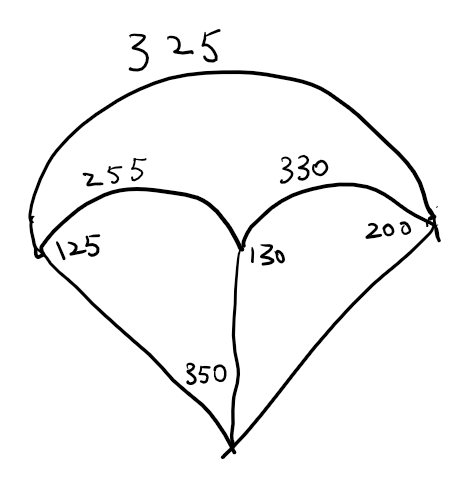
\includegraphics[scale=0.5]{hku-ccst9017-assignment-4-img-001}



% --------------------------------------------------------------
%     You don't have to mess with anything below this line.
% --------------------------------------------------------------

\end{document}